\secput{intro}{Introduction}

The \defn{predecessor} problem is to find the largest item in a given sorted list $L$
that is not greater than a query value $q \in \mathbb{R}$.  The \defn{iterated predecessor query} 
problem is to find the predecessor for a query $q$ in each of a set of $k$ static lists
$L_1 \ldots L_k$, each of size $n$.  A naive solution involves individual binary searches over all
$k$ lists, which would require $O(k \lg n)$ time in the worst-case.  However, Chazelle
and Guibas~\cite{ChazelleGu86a} showed that the lists can be 
preprocessed to support iterated predecessor queries in $O(\lg n + k)$ time, with
linear preprocessing time and linear space via their technique \defn{fractional cascading}.

In this project, we will demonstrate that the iterated predecessor query problem
can also be solved using a technique called \defn{range coalescing} in $O(\lg n + k)$ time.
Range coalescing is \defn{cache-oblivious}~\cite{FrigoLePr99}, using only 
$O(\log_{B+1} n + k/B)$ memory transfers per query in the worst case.\footnote{Throughout 
this paper we will use the notation $\lg n$ to mean $\log_2 n$ and $\ln n$ to 
mean the natural logarithm.}  Furthermore, range coalescing requires
only linear space and the preprocessing requires $O(kn)$ time and $O(kn/B)$ memory
transfers.

The essence of range coalescing, as the name suggests, is to coalesce ranges of 
the query space into $n$ ''bins'', each of which could generate $O(k)$ different results
depending on the specific value of $q$ within that range.
\figref{range_coalescing} illustrates how the smallest element in each bin has 
is the ''splitter'' for the bin, so named because they collectively ''split'' all
of the elements into bins of contiguous value ranges.  In addition,
the predecessor of the splitter from each list is included in order to
service predecessor requests that are smaller in value than the smallest element
in the bin from each list.  \figref{coalesced_bin} gives an example of how the data
in a bin is stored.  The elements from each list are stored in sorted subsequences of
varying lengths, but of total length $O(k)$. Each bin stores $O(k)$ different 
values and thus the total data structure is linear space.

A query $q$ on a bin $D$ walks through the $O(k)$ elements in $D$ in a single pass.
Within $D$ are $k$ subsequences of each list in sorted order as depicted in 
\figref{coalesced_bin}, so we merely take the
largest element from the $i$th subsequence which is not larger than $q$ as our predecessor
answer from the $i$th list.  A more detailed description of the query process can
be found in \secref{solution}.

\begin{figure}[h]
%\begin{center}
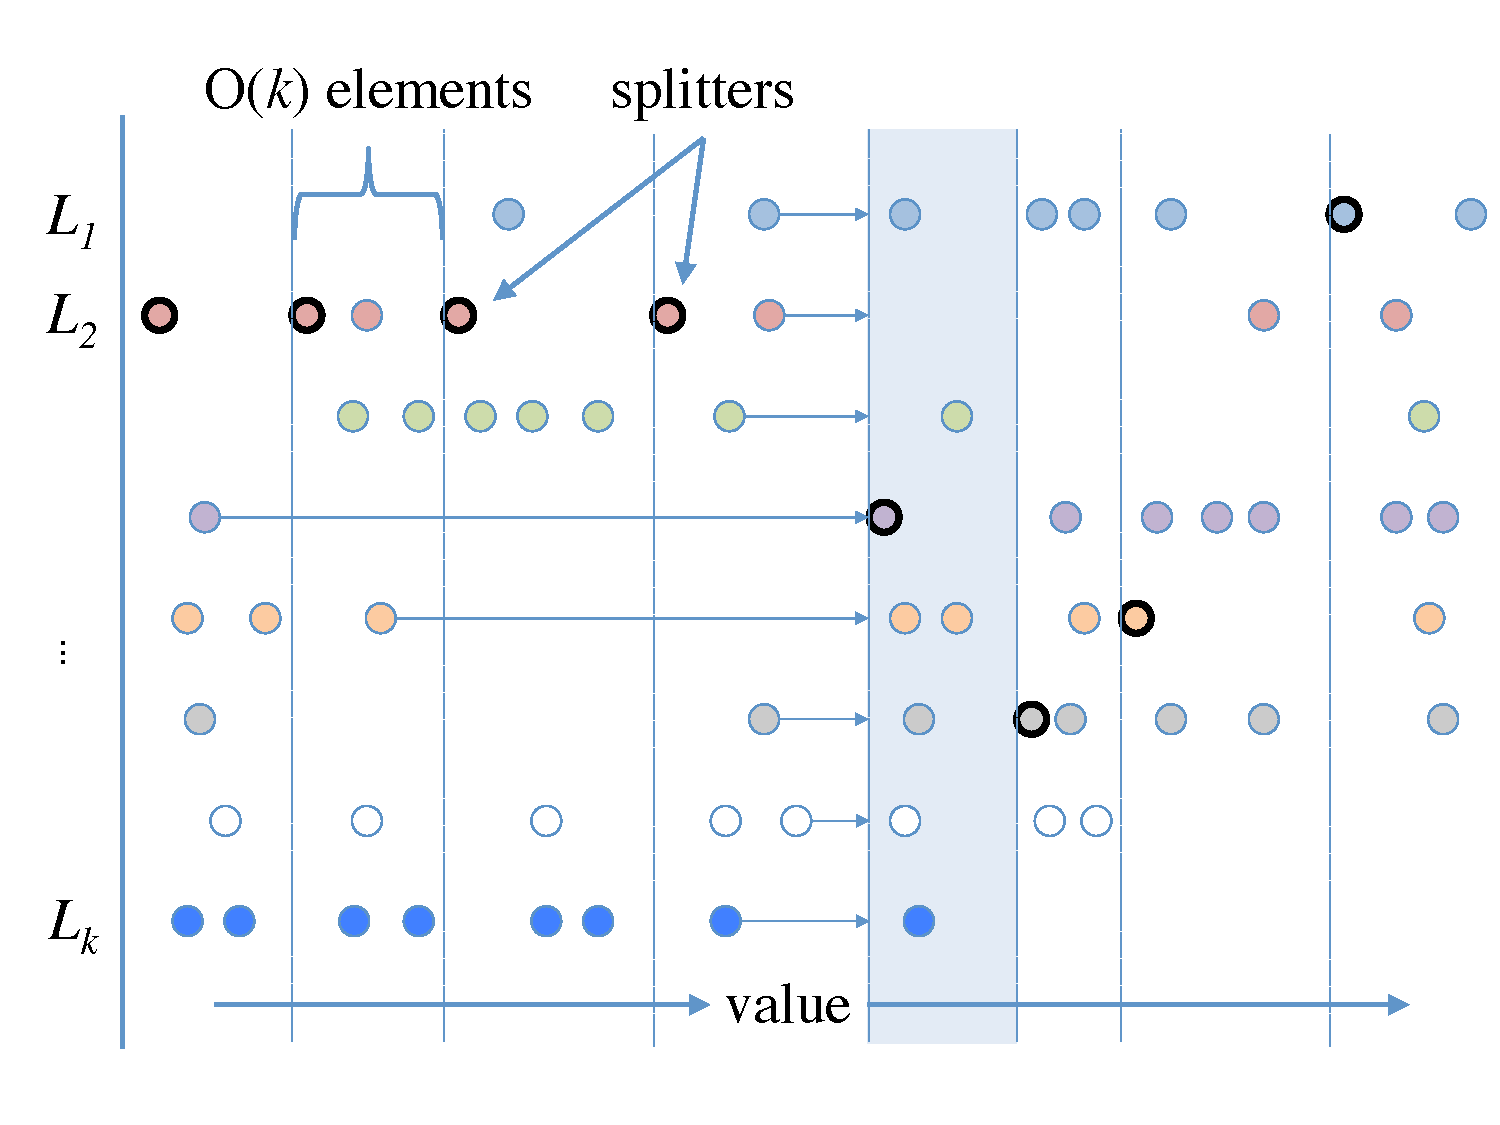
\includegraphics[scale=.3]{cache-oblivious-fractional-cascading-a.pdf}
%\end{center}
\caption{Range coalescing data structure for the iterated predecessor problem with
the value of the element on the $x$-axis and each row representing a list in 
$\{ L_1 \ldots L_k \}$.
Each vertical line delineates the $O(k)$ elements in each bin.  The elements with a heavy
black border are the splitters for each bin --- the smallest item in the bin is
the splitter.  An example bin is highlighted by the blue vertical bar.  The elements
to the left of the bar with rightward arrows are the predecessors of the splitter
from the blue bin in each list.}
\label{fig:range_coalescing} 
\end{figure}

\begin{figure}[h]
%\begin{center}
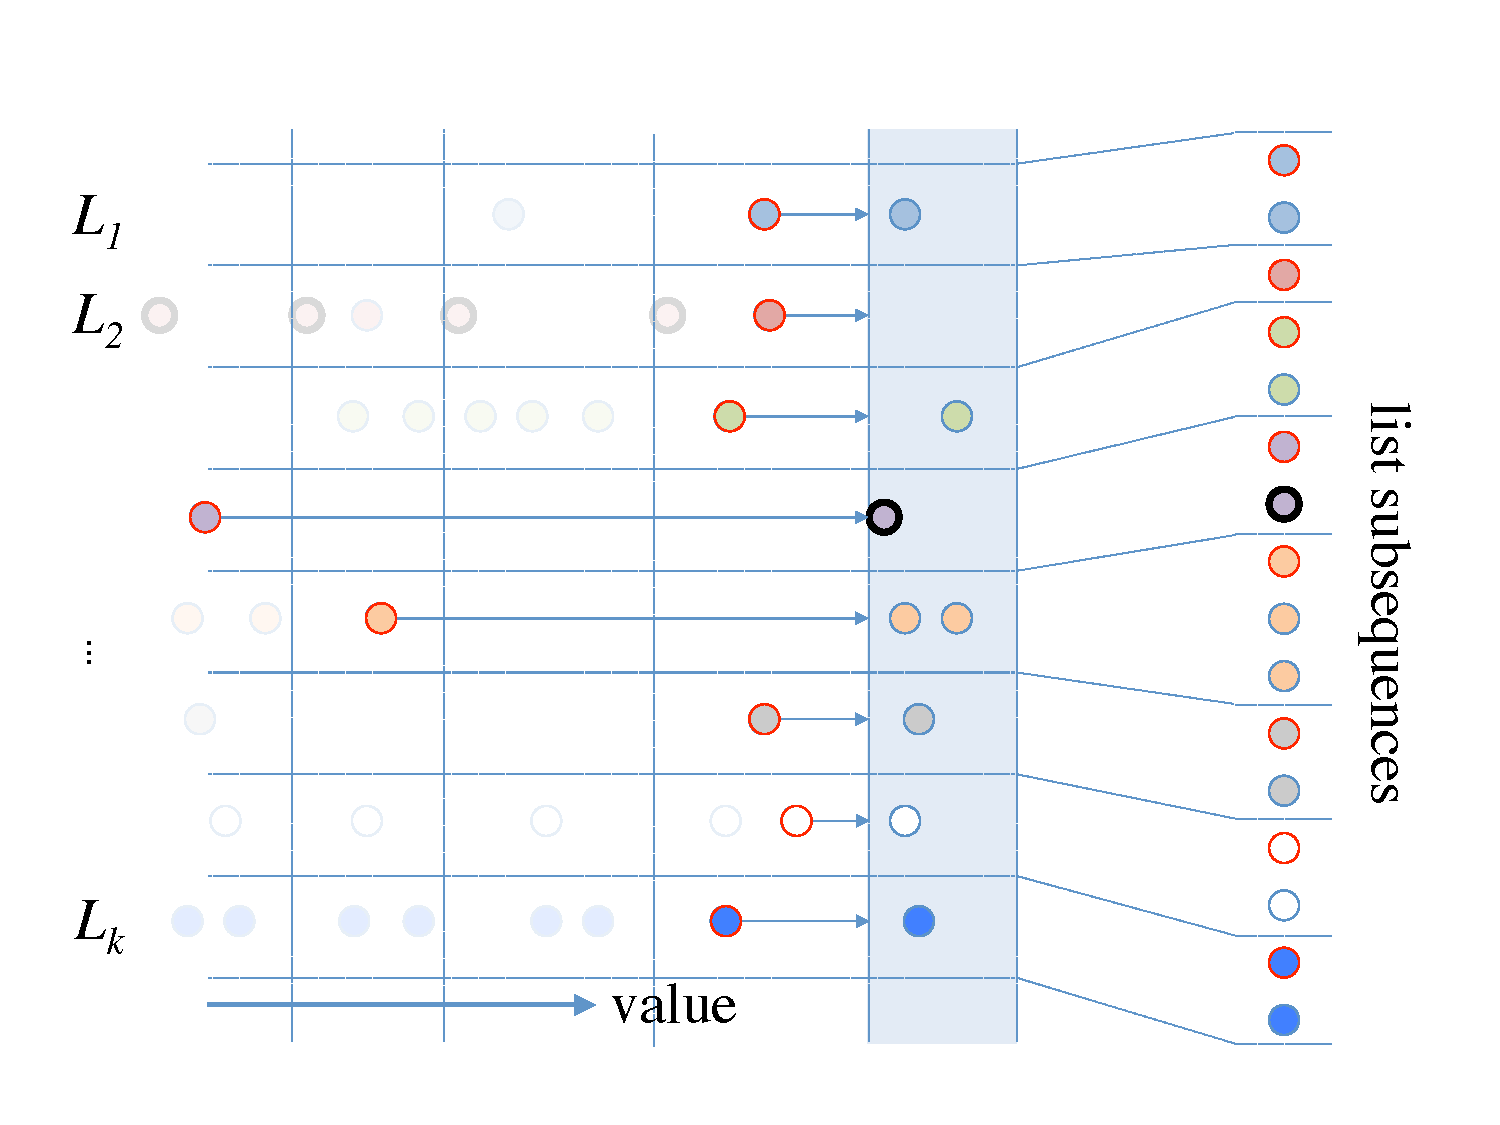
\includegraphics[scale=.33333]{cache-oblivious-fractional-cascading-c.pdf}
%\end{center}
\caption{An example of how a bin is constructed in a range coalescing data
structure.  The elements that fall in the range of the blue bar and the predecessor
of the splitter (with heavy black border) from each list is represented in the bin.
In particular, the subsequences of those elements from each list are stored together
and concatenated so that the subsequence from $L_1$ comes first and so on until the
subsequence from $L_k$.}
\label{fig:coalesced_bin} 
\end{figure}

Throughout this paper we will let $M$ be the size of the cache and $B$ be the size
of the cache blocks
on a hypothetical external memory machine.  We will consider solutions to the iterated
predecessor problem, in which we are given $k$ $n$-length lists $L_1 \ldots L_k$ and
we preprocess them to improve the query time.

In \secref{cacheoblivious} we discuss some simple known results from the study of
cache-oblivious algorithms and data structures which are useful in subsequent analysis.
\secref{simple} gives an overview of solutions to the iterated predecessor problem
which are not cache-oblivious, but nonetheless serve as a reasonable baseline for
our work.  We present range coalescing in \secref{solution} and show that they
answer queries cache-obliviously using $O(\log_{B+1} n + k/B)$ memory transfers.
\secref{preprocessing} demonstrates that the preprocessing for a range coalescing
data structure requires only $O(kn/B)$ with high probability.  \secref{results} 
describes our implementations of each solution described herein and an experimental
methodology for testing the performance of each.  Finally, \secref{conclusion} 
describes some limitations of range coalescing, providing opportunities for future
work.

